\documentclass[hyperref={pdfpagelabels=false,linkcolor=blue}, aspectratio=1610]{beamer}
\usepackage{color}						% Text coloring
\usepackage[normalem]{ulem}			% Strike out with \sout
\usepackage{amsmath, amsthm, amssymb, cancel} % More math options
\usepackage{varioref}					% Defines \vref
\usepackage{multimedia}					% Include videos and multimedia
\usepackage{booktabs} 					% Nicer tables
\usepackage{tabularx}					% Nicer tables
% Fonten som IEEE conf bruker i \mathscr er lik den vanlige \mathscr som trenger pakken mathrsfs
\usepackage{mathrsfs}
% Bruk eventuelt replace \mathscr med \mathscr

%Hindrer warning om fontstørrelse
\let\Tiny=\tiny
% Hindrer beamer i å gjøre replacement av fonts. 
% Dette hindrer at beamer "ødelegger" matematiske formler ved å bytte ut "løkkeskrift-funksjons" f, med en vanlig f.
\usefonttheme{professionalfonts}
%\usefonttheme[onlymath]{serif}
%\usepackage{times}
%\DeclareMathAlphabet{\mathscr}{OMS}{cmsy}{m}{n}

\usepackage{default}
\usepackage{xcolor}
\usepackage[utf8]{inputenc}
\usepackage{lmodern}
\usepackage{xspace}
\usepackage{etex}
\usepackage{pgfpages}
\usepackage{graphicx}

% \reserveinserts{50}
\usepackage{tikz}

\usetikzlibrary{arrows}
\usepgflibrary{shapes.geometric}
\usepgflibrary{shapes.arrows}
\usetikzlibrary{fit}
\usetikzlibrary{backgrounds}
\usepgflibrary{shapes.misc}
\usepgflibrary{shapes.callouts}
\usetikzlibrary{shapes.callouts}
\usetikzlibrary{positioning}

\newcommand{\pname}[1]{\ensuremath{\langle \textsf{#1} \rangle}}

\newcommand\blfootnote[1]{%
  \begingroup
  \renewcommand\thefootnote{}\footnote{#1}%
  \addtocounter{footnote}{-1}%
  \endgroup
}

\useoutertheme[width=2cm]{sidebar}

\makeatletter
\setbeamertemplate{sidebar left}{%
  \vspace*{\fill}
  
\includegraphics[width=1.82cm,height=7.99cm]{uis-sidebar.jpg}\par
  \vfill
  \parbox{1.5cm}{\centering\textcolor{black}{}}
  \vspace*{0.6cm}
}
\makeatother

\useoutertheme[subsection=false, footline=institutetitle]{miniframes}

\def\insertframetitle{}
\makeatletter
\setbeamertemplate{headline}{}
\setbeamertemplate{frametitle}
{
\vskip10pt
\LARGE\textbf \insertframetitle \hfill
\vspace*{-0.3cm}
 \begin{beamercolorbox}[colsep=0.5pt]{lower separation line head}
 \end{beamercolorbox}
}
\makeatother

% Modify colors of headlines
\definecolor{beamer@uisblue}{cmyk}{1,0.6,0,0.4} % changed this
\setbeamercolor{upper separation line head}{bg=white}
\setbeamercolor{middle separation line head}{bg=white}
\setbeamercolor{lower separation line head}{bg=white}
\setbeamercolor{upper separation line foot}{bg=beamer@uisblue}
\setbeamercolor{lower separation line foot}{bg=white}
\setbeamercolor{frametitle}{fg=beamer@uisblue}
\setbeamercolor{section in head/foot}{fg=beamer@uisblue}
\setbeamercolor{structure}{fg=beamer@uisblue}

% Font size, set larger fontsizes to limit amount of text on slides
\setbeamerfont*{normal text}{size=\LARGE}
\setbeamerfont*{title in head/foot}{size=\tiny}
\setbeamerfont*{section in head/foot}{size=\scriptsize}
\setbeamerfont*{block title}{size=\LARGE}
\setbeamerfont*{block body}{size=\Large}
\setbeamerfont*{itemize/enumerate body}{size=\Large}
\setbeamerfont*{itemize/enumerate subbody}{size=\large}
\setbeamerfont*{title}{size=\LARGE}
\setbeamerfont*{title page}{size=\large}
\setbeamerfont*{subtitle}{size=\Large}

% Remove navigation symbols
\setbeamertemplate{navigation symbols}{}

\makeatletter
\newcommand*{\compresson}{\addtocontents{nav}{\protect\headcommand{\protect\beamer@compresstrue}}}
\newcommand*{\compressoff}{\addtocontents{nav}{\protect\headcommand{\protect\beamer@compressfalse}}}
\makeatother



\title[Thesis Writing]{Introduction to Writing a PhD Thesis}
\subtitle{Publishing, Tips, Tools, and Recommendations}
\author[Hein Meling]{{\bf Hein Meling}}
\institute[Univ. of Stavanger]
	{
\includegraphics[scale=0.4]{./uis-logo-en.pdf}
	\\{\emph{hein.meling@uis.no}}}
\date[Dec 2018]{December 2018}

\begin{document}

\compresson

% Use \hoffset to center text on a title page without sidebar
\begingroup
\makeatletter
\setlength{\hoffset}{-.5\beamer@sidebarwidth}
\makeatother
\begin{frame}[plain]
    \titlepage
\end{frame}
\endgroup

\begin{frame}
\frametitle{Planning Your Thesis Work}
\begin{block}{}
 \begin{itemize}
  \item 3 Years fly by; Not a whole lot of time!
  \item Need careful planning
  \item Important to stay focused
 \end{itemize}
\end{block}
\end{frame}

\begin{frame}
\frametitle{Research Proposal}
\begin{block}{}
 \begin{itemize}
  % \item During the first semester, while taking courses you need to prepare a research proposal
  	\item Background and Motivation
	\begin{itemize}
		\item What are the problems you target?
	\end{itemize}
	\item Project Description
	\begin{itemize}
		\item Objectives / Research Questions
	\end{itemize}
	\item Research Methodologies to use
	\item Progress Plan
	\begin{itemize}
		\item Planned publications:\\
		topic and related to which research questions
		\item Gantt Chart with Tasks and Milestones
	\end{itemize}
	\item Course Plan
	\item Mobility
  % \item Submit research proposal by \textbf{Monday December 3, 2018}
 \end{itemize}
\end{block}
\end{frame}

\begin{frame}
\frametitle{Gantt Chart}
 \begin{center}
  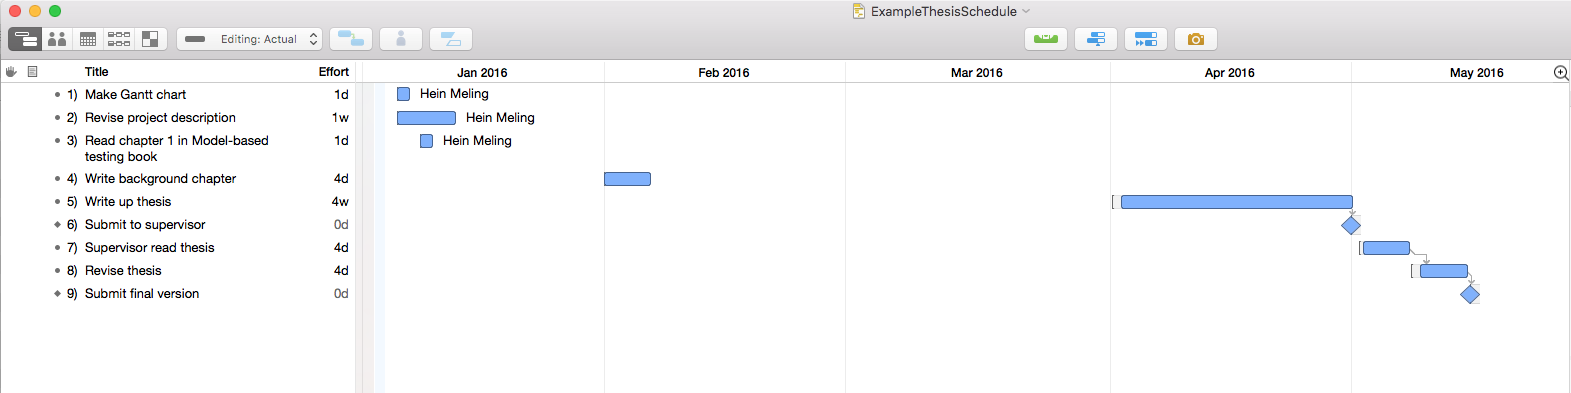
\includegraphics[scale=0.25]{fig/gantt-example}
 \end{center}
\end{frame}

\begin{frame}
\frametitle{When Attending a Conference or S/W School}
\begin{block}{}
 \begin{itemize}
  \item Make connections
  \begin{itemize}
  	\item At least 5 other students / 3 speakers/professors
  \end{itemize}
  \item Tell them your plans and ideas and solicit their feedback.
  \begin{itemize}
  	\item Prepare a pitch; a few representative and memorable sentences
  \end{itemize}
  \item Make notes about their research/personal interests in a journal (include their picture).
  \item Don't do it while talking with them, but afterwards, as soon as it is appropriate.
  \item Then next time you have a chance to meet them (the next conference), read your notes before traveling. You give a good impression that you remembered them. They will start to remember you!
 \end{itemize}
\end{block}
\end{frame}

\begin{frame}
\frametitle{Publishing}
\begin{block}{}
 \begin{itemize}
  \item Target top conferences
  \item Better to have 1 strong publication at a top conference 
        than 4 at low-tier conferences
  \item People will look at where you published
  \item In Computer Science (systems), ACM and USENIX venues often considered more prestigious than IEEE; there are some exceptions of course
  \item \textbf{Better to take a few rejects than to submit to easy places}
 \end{itemize}
\end{block}
\end{frame}

\begin{frame}
\frametitle{Publishing: Plan the Process}
\begin{block}{}
 \begin{itemize}
  \item Pick target conference (deadline given)
  \item Set milestones for intermediate results and subgoals
  \item Timeframe between 3-6 months
  \item Again: use Gantt chart
  \item Revise plan once every two weeks (approx)
 \end{itemize}
\end{block}
\end{frame}

\begin{frame}
\frametitle{Paper Writing Resources (Youtube)}
\begin{block}{}
 \begin{itemize}
  \item \href{https://www.youtube.com/watch?v=UY7sVKJPTMA&feature=share}{How to Write a Paper in a Weekend}\\(By Prof. Pete Carr)
  \item \href{https://youtu.be/1AYxMbYZQ1Y}{PhD: How to write a great research paper}\\(By Simon Payton Jones)
  \item \href{https://youtu.be/OV5J6BfToSw}{Linguistics, Style and Writing in the 21st Century - with Steven Pinker}
 \end{itemize}
\end{block}
\end{frame}

\begin{frame}
\frametitle{Writing a Systems Paper (Links)}
\begin{block}{}
 \begin{itemize}
  \item \href{http://gramoli.redbellyblockchain.io/web/doc/talks/researchmethod.pdf}{How to write a systems paper}
  \item  \href{https://www.doc.ic.ac.uk/~prp/doc/talks/11-prp-paper_writing.pdf}{How To Get Your Systems Paper Accepted?}
  \item \href{http://www.cse.unsw.edu.au/~gernot/talk-howto-paper.pdf}{How to Write a Good Paper}
  \item  \href{http://www.cse.unsw.edu.au/~gernot/benchmarking-crimes.html}{Systems Benchmarking Crimes}
  \item \href{http://www.cse.unsw.edu.au/~gernot/style-guide.html}{Tips and Guidance for Students Writing Papers and Reports}
 \end{itemize}
\end{block}
\end{frame}

\begin{frame}
\frametitle{Books}
\begin{block}{}
 \begin{itemize}
  \item The Elements of Style
  \item Writing for Scholars
  \item Forskerhåndboken
 \end{itemize}
\end{block}
\end{frame}

\begin{frame}
\frametitle{Work Process}
\begin{block}{}
 \begin{itemize}
  \item Individual meetings (approx. 1 hour)
  \item Group meetings (approx. 2 hours)
  \item Reading group (approx. 1 hour)
 \end{itemize}
\end{block}
\end{frame}

\begin{frame}
\frametitle{Conference Schedule}
 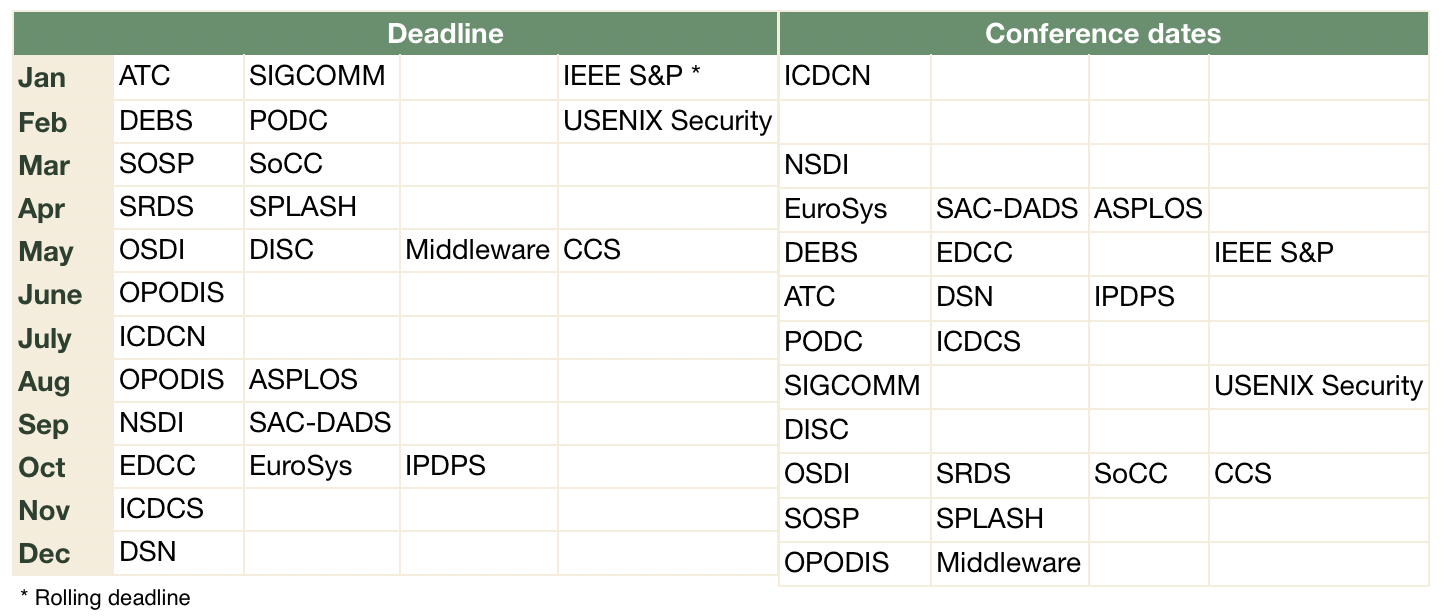
\includegraphics[scale=0.25]{fig/ConferenceSchedule.png}
\end{frame}

\begin{frame}
\frametitle{When to Start Writing?}
\begin{block}{}
 \begin{itemize}
  \item<2-> Today!
  \item<2-> You can set up the document 
  \item<2-> Prepare a disposition (fill in the headings)
  \item<2-> You can always change things later
 \end{itemize}
\end{block}
\end{frame}

\begin{frame}
\frametitle{How To Structure the Thesis Report}
\begin{block}{}
 % Talk to each bullet here:
 \begin{itemize}
  \item Abstract (300-500 words)
  \item Introduction (3-5 pages)
  \begin{itemize}
  	\item Motivate why your topic is important; summarize idea and results
	\item Important chapter
  \end{itemize}
  % Explain that intro is important; it is what makes the reader decide if it is worth their time
  \item Background, Technology Review, Related Work (10-20 p.)
  % Explain difference between background and related work
  \item Design, Model, Architecture (10-30 p.)
  \item Implementation (10-20 p.)
  \begin{itemize}
   \item Technical details of interest, optimizations, algorithms, ...
   \item Don't explain every bit of code; only the interesting parts
  \end{itemize}
  \item Evaluation, Discussion, Insights (10-30 p.)
  \item Conclusion (300-500 words)
  \begin{itemize}
  	\item Tie the results back to what you promised in the introduction
  \end{itemize}
 \end{itemize}
\end{block}
\end{frame}

\begin{frame}
\frametitle{Tips for Thesis or Paper}
\begin{block}{}
 \begin{itemize}
  \item Name chapters appropriately; other names than those on previous slide is ok.
  \item Start Chapter/Section with a brief summary of what the reader can expect to learn from reading it.
  \begin{itemize}
   \item Thus far, we have presented Replacement for a single Paxos instance. In this section, we explain how to apply Replacement to an RSM that executes a sequence of Paxos instances.
  \end{itemize}
  \item Insert paragraph breaks (avoid too long paragraphs)
  \item No spelling mistakes (use spellchecker!)
  \item Reasonable formatting; it should look nice!
 \end{itemize}
\end{block}
\end{frame}

\begin{frame}
\frametitle{How to Work?}
\begin{block}{}
 \begin{itemize}
  \item<2-> Switch between coding and writing!
  \item<2-> Expect to rewrite everything you write; 
  \begin{itemize}
  	\item<2-> So don't spend time making it perfect 
  \end{itemize}
  \item<2-> Iterate to improve report to make it perfect
  \item<2-> Why work this way?
  \begin{itemize}
	\item<2-> Two modes of thinking
  	\item<2-> Makes you think differently about the problem 
  \end{itemize}
 \end{itemize}
\end{block}
\end{frame}

\begin{frame}
\frametitle{Specification: Thinking Before Coding}
\begin{block}{}
 \begin{itemize}
  \item Write specifications:
  \begin{itemize}
  	\item high-level specification of system
	\item low-level specification for each function
  \end{itemize}
  \item Textual specifications are fine!
  \item Also: Express ideas in diagrams and figures
  \item Simplicity
 \end{itemize}
\end{block}
\end{frame}

\begin{frame}
\frametitle{Modeling Languages}
\begin{block}{}
 \begin{itemize}
  \item Unified Modeling Language (UML)
  \begin{itemize}
	\item Use Case Diagrams
  	\item \textbf{Class Diagrams} (Entity Relation)
	\item \textbf{Sequence Charts}
	\item \textbf{State Machine Diagrams}
  \end{itemize}
  \item \textbf{Flow Charts}
  \item Work Flow Diagrams
  \item Data Flow Diagrams
  \item Wireframe / UI Mockups
  \item Infographics
 \end{itemize}
\end{block}
\end{frame}

\begin{frame}
\frametitle{Tools}
\begin{block}{}
 \begin{itemize}
  \item git and github
  \item Dropbox
  \item LaTeX/bibtex for the report
  \item Slack for chat rooms
 \end{itemize}
\end{block}
\end{frame}

\begin{frame}
\frametitle{Quick Guide to git Command Line}
\begin{block}{}
 \begin{itemize}
  \item git clone \pname{repo-link from github}
  \item git add \pname{new-file}
  \item git commit \quad (supply commit message)
  \item git push \quad (send changes to github)
  \item git fetch --all \quad (get changes from github, e.g. by other team members)
  \item git merge \quad (merge changes from github with local branch)
 \end{itemize}
\end{block}
\end{frame}

\begin{frame}
\frametitle{Quick Guide to git Command Line}
\begin{block}{}
 \begin{itemize}
  \item git pull \quad (alternative to fetch and merge, but causes merge commits that distort the history of changes when not necessary)
  \item git diff \quad (view your changes before commit)
  \item git diff --word-diff \quad (view your changes before commit)
  \item git log \quad (see log of all commits)
 \end{itemize}
\end{block}
\end{frame}

\begin{frame}
\frametitle{Best Practices: GitHub and LaTeX}
\begin{block}{}
 \begin{itemize}
  \item Naming folders (under bbchain repo):
  \begin{itemize}
  	\item consistent naming; lower-case; think of a good name!
	\item papers/\pname{project-name}/\pname{conference-name}
	\item Example: papers/blockchain-storage/icdcs2020
  \end{itemize}
  \begin{itemize}
  	\item In root folder:
	\begin{itemize}
		\item main.tex
		\item main.bib
		\item \pname{template files for conference/journal}
		\item .gitignore \quad (Use GitHub's TeX template)
	\end{itemize}
	\item In subfolders:
	\begin{itemize}
		\item tex/ \quad fig/ \quad alg/ \quad plots/
	\end{itemize}
	\item Do not commit generated files, including main.pdf
	\begin{itemize}
		\item Include such files in .gitignore
	\end{itemize}
  \end{itemize}
  \end{itemize}
\end{block}
\end{frame}

\begin{frame}
\frametitle{Conclusions}
\begin{block}{}
 \begin{itemize}
  \item We have high expectations
  \item We want you to succeed!
 \end{itemize}
\end{block}
\end{frame}

\end{document}
